\Cref{fig:sweep} and \cref{tab:sweep} give torque, axial pull and stator flux linkage from 0 to \SI{300}{A} on the $q$ axis, together with the effect of current advance at \SI{250}{A}. The no-load flux linkage is $\psi_m=\SI{8.62}{mWb}$, so the linear torque constant is $\frac32 p\psi_m=\SI{0.194}{\newton\metre\per\ampere}$. At \SI{250}{A} the 3-D torque is 86\,\% of the linear value, and at \SI{300}{A} it is 80\,\%: saturation, not magnet strength, sets the peak torque. Unlike a steel-backed rotor, the axial pull falls with $q$-axis current, because armature reaction weakens the main flux under half of each pole. Current advance reduces torque monotonically, so the maximum-torque-per-ampere angle is close to the $q$ axis.
\begin{figure*}[!t]\centering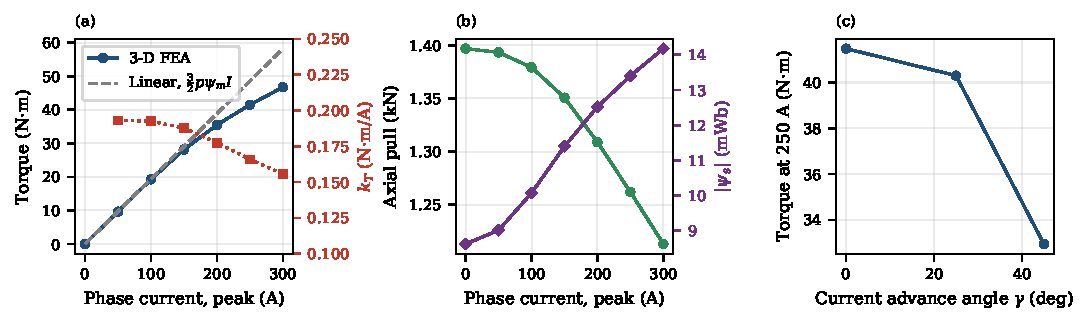
\includegraphics[width=\textwidth]{sweep.pdf}
\caption{TREN-V4 v4b performance from the 3-D model. (a) Torque and torque constant against $q$-axis current, with the linear (unsaturated) extrapolation; (b) axial magnetic pull and stator flux-linkage magnitude; (c) torque against current advance angle at \SI{250}{A}.}\label{fig:sweep}\end{figure*}
\begin{table}[!t]\caption{3-D results against $q$-axis current (v4b, ideal materials)}\label{tab:sweep}\centering\footnotesize
\begin{tabular}{@{}rrrrr@{}}\toprule $I$ (A) & $T$ (\Nm) & $k_T$ (\Nm/A) & $F_z$ (kN) & $|\psi_s|$ (mWb)\\\midrule
0 & 0.03 & -- & 1.40 & 8.62\\
50 & 9.66 & 0.193 & 1.39 & 9.01\\
100 & 19.26 & 0.193 & 1.38 & 10.07\\
150 & 28.16 & 0.188 & 1.35 & 11.40\\
200 & 35.48 & 0.177 & 1.31 & 12.52\\
250 & 41.48 & 0.166 & 1.26 & 13.40\\
300 & 46.72 & 0.156 & 1.21 & 14.18\\
\bottomrule\end{tabular}\end{table}
